\let\negmedspace\undefined
\let\negthickspace\undefined
\documentclass[journal]{IEEEtran}
\usepackage[a5paper, margin=10mm, onecolumn]{geometry}
%\usepackage{lmodern} % Ensure lmodern is loaded for pdflatex
\usepackage{tfrupee} % Include tfrupee package

\setlength{\headheight}{1cm} % Set the height of the header box
\setlength{\headsep}{0mm}     % Set the distance between the header box and the top of the text

\usepackage{gvv-book}
\usepackage{gvv}
\usepackage{cite}
\usepackage{amsmath,amssymb,amsfonts,amsthm}
\usepackage{algorithmic}
\usepackage{graphicx}
\usepackage{textcomp}
\usepackage{xcolor}
\usepackage{txfonts}
\usepackage{listings}
\usepackage{enumitem}
\usepackage{mathtools}
\usepackage{physics}
\usepackage{gensymb}
\usepackage{comment}
\usepackage[breaklinks=true]{hyperref}
\usepackage{tkz-euclide} 
\usepackage{listings}
% \usepackage{gvv}                                        
\def\inputGnumericTable{}                                 
\usepackage[latin1]{inputenc}                                
\usepackage{color}                                            
\usepackage{array}                                            
\usepackage{longtable}                                       
\usepackage{calc}                                             
\usepackage{multirow}                                         
\usepackage{hhline}                                           
\usepackage{ifthen}                                           
\usepackage{lscape}
\begin{document}

\bibliographystyle{IEEEtran}
\vspace{3cm}

\title{2.7.30}
\author{EE25BTECH11018 - DARISY SREETEJ}
% \maketitle
% \newpage
% \bigskip
{\let\newpage\relax\maketitle}

\renewcommand{\thefigure}{\theenumi}
\renewcommand{\thetable}{\theenumi}
\setlength{\intextsep}{10pt} % Space between text and floats


\numberwithin{equation}{enumi}
\numberwithin{figure}{enumi}
\renewcommand{\thetable}{\theenumi}


\textbf{Question}:
 Find the value of $k$ so that the area of $\triangle$$ABC$ with $\vec{A}\brak{k+1,1}$ , $\vec{B}\brak{4,-3}$ and $\vec{C}\brak{7, -k}$ is $6$ square units

\quad

\textbf{Solution:}
\\
Given,
\begin{align}
    \vec{A}=\myvec{k+1\\1}\\
    \vec{B}=\myvec{4\\-3}\\
    \vec{C}=\myvec{7\\-k}
\end{align}
Now, consider 
\begin{align}
\vec{AB}= \vec{B}-\vec{A}=\myvec{4\\-3} - \myvec{k+1\\1} = \myvec{3-k\\-4}\\
\vec{AC}= \vec{C}-\vec{A}= \myvec{7\\-k} - \myvec{k+1\\1} = \myvec{6-k\\-k-1}
\end{align}
The Area of the $\triangle$$ABC$ :
\begin{align}
\text{Area\brak{\triangle ABC}}&=\frac{1}{2}\norm{\brak{\vec{B}-\vec{A}}\times\brak{\vec{C}-\vec{A}}}. 
\end{align}
Here according to problem , the Area of $\triangle$$ABC$ is $6$ square units\\
Therefore,
\begin{align}
\frac{1}{2}\norm{\brak{\vec{B}-\vec{A}}\times\brak{\vec{C}-\vec{A}}}=6\\
\frac{1}{2}\norm{\myvec{3-k\\-4}\times\myvec{6-k\\-k-1}}=6
\end{align}
\begin{align}
\mdet{\brak{3-k}\brak{-k-1} - \brak{-4}\brak{6-k}}=12 \\
\mdet{k^2-6k+21}=12
\end{align}
Case 1 :
\begin{align}
   k^2-6k+24=12\\
k^2-6k+9=0\\
(k-3)^2=0\\
k=3
\end{align}
Case 2 :
\begin{align}
k^2-6k+24=-12\\
k^2-6k+33=0\\
\end{align}
Discriminant: $D=-96$.\\ Since the discriminant is negative , there is no real solution for this case.\\

Thus , k=3
\begin{figure}[h!]
    \centering
    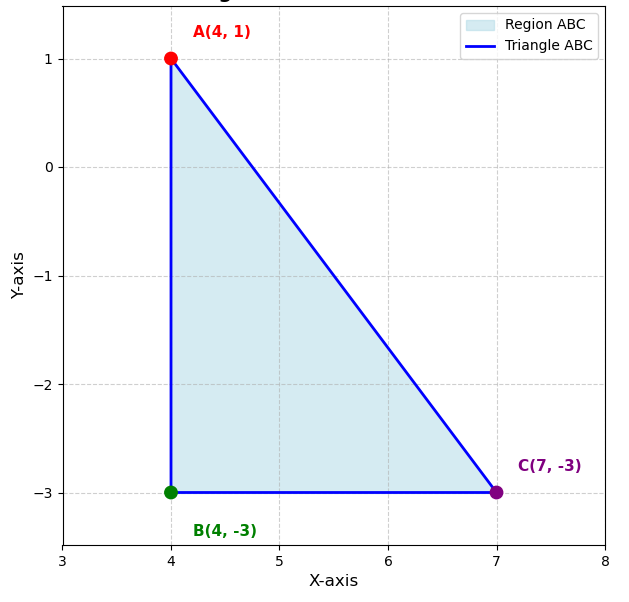
\includegraphics[width=0.7\columnwidth]{figs/fig.png}
    \caption*{Fig: $\triangle$$ABC$ with shaded area}
    \label{fig:placeholder}
\end{figure}
\end{document}  
